\documentclass[11pt]{charter}

% El títulos de la memoria, se usa en la carátula y se puede usar el cualquier lugar del documento con el comando \ttitle
\titulo{Sistema de control y monitoreo de confort y consumo energético para viviendas y edificios} 

% Nombre del posgrado, se usa en la carátula y se puede usar el cualquier lugar del documento con el comando \degreename
%\posgrado{Carrera de Especialización en Sistemas Embebidos} 
\posgrado{Carrera de Especialización en Internet de las Cosas} 
%\posgrado{Carrera de Especialización en Intelegencia Artificial}
%\posgrado{Maestría en Sistemas Embebidos} 
%\posgrado{Maestría en Internet de las cosas}

% Tu nombre, se puede usar el cualquier lugar del documento con el comando \authorname
\autor{Daniel Iván Cruz Flores} 

% El nombre del director y co-director, se puede usar el cualquier lugar del documento con el comando \supname y \cosupname y \pertesupname y \pertecosupname
\director{Nombre del Director}
\pertenenciaDirector{pertenencia} 
% FIXME:NO IMPLEMENTADO EL CODIRECTOR ni su pertenencia
\codirector{} % si queda vacio no se deberíá incluir 
\pertenenciaCoDirector{}

% Nombre del cliente, quien va a aprobar los resultados del proyecto, se puede usar con el comando \clientename y \empclientename
\cliente{Emprendimiento Personal}
\empresaCliente{Emprendimiento Personal}

% Nombre y pertenencia de los jurados, se pueden usar el cualquier lugar del documento con el comando \jurunoname, \jurdosname y \jurtresname y \perteunoname, \pertedosname y \pertetresname.
\juradoUno{Nombre y Apellido (1)}
\pertenenciaJurUno{pertenencia (1)} 
\juradoDos{Nombre y Apellido (2)}
\pertenenciaJurDos{pertenencia (2)}
\juradoTres{Nombre y Apellido (3)}
\pertenenciaJurTres{pertenencia (3)}
 
\fechaINICIO{25 de agosto de 2020}		%Fecha de inicio de la cursada de GdP \fechaInicioName
\fechaFINALPlanificacion{0 de mes de 2020} 	%Fecha de final de cursada de GdP
\fechaFINALTrabajo{0 de mes de 2020}		%Fecha de defensa pública del trabajo final


\begin{document}

\maketitle
\thispagestyle{empty}
\pagebreak


\thispagestyle{empty}
{\setlength{\parskip}{0pt}
\tableofcontents{}
}
\pagebreak


\section{Registros de cambios}
\label{sec:registro}


\begin{table}[ht]
\label{tab:registro}
\centering
\begin{tabularx}{\linewidth}{@{}|c|X|c|@{}}
\hline
\rowcolor[HTML]{C0C0C0} 
Revisión & \multicolumn{1}{c|}{\cellcolor[HTML]{C0C0C0}Detalles de los cambios realizados} & Fecha      \\ \hline
1.0      & Creación del documento                                          & 27/06/2020 \\ \hline
1.1      &                                                                 & dd/mm/aaaa \\ \hline
1.2      & Otro ejemplo \newline
		   Con texto partido \newline
		   En varias líneas \newline
		   A propósito                                                     & dd/mm/aaaa \\ \hline
\end{tabularx}
\end{table}

\pagebreak



\section{Acta de constitución del proyecto}
\label{sec:acta}

\begin{flushright}
Buenos Aires, \fechaInicioName
\end{flushright}

\vspace{2cm}

Por medio de la presente se acuerda con el Ing. \authorname\hspace{1px} que su Trabajo Final de la \degreename\hspace{1px} se titulará ``\ttitle'', consistirá esencialmente en el prototipo preliminar de un sistema capaz de controlar y monitorear viviendas u otros ambientes mediante el protocolo MQTT para brindar una gestión inteligente respecto a confort y consumo energético, y tendrá un presupuesto preliminar estimado de 600 hs de trabajo y \textcolor{red}{\$XXX}, con fecha de inicio \fechaInicioName\hspace{1px} y fecha de presentación pública \fechaFinalName.

Se adjunta a esta acta la planificación inicial.

\vfill

% Esta parte se construye sola con la información que hayan cargado en el preámbulo del documento y no debe modificarla
\begin{table}[ht]
\centering
\begin{tabular}{ccc}
\begin{tabular}[c]{@{}c@{}}Ariel Lutenberg \\ Director posgrado FIUBA\end{tabular} & \hspace{2cm} & \begin{tabular}[c]{@{}c@{}}\clientename \\ \empclientename \end{tabular} \vspace{2.5cm} \\ 
\multicolumn{3}{c}{\begin{tabular}[c]{@{}c@{}} \supname \\ Director del Trabajo Final\end{tabular}} \vspace{2.5cm} \\
%\begin{tabular}[c]{@{}c@{}}\jurunoname \\ Jurado del Trabajo Final\end{tabular}     &  & \begin{tabular}[c]{@{}c@{}}\jurdosname\\ Jurado del Trabajo Final\end{tabular}  \vspace{2.5cm}  \\
%\multicolumn{3}{c}{\begin{tabular}[c]{@{}c@{}} \jurtresname\\ Jurado del Trabajo Final\end{tabular}} \vspace{.5cm}                                                                     
\end{tabular}
\end{table}




\section{Descripción técnica-conceptual del proyecto a realizar}
\label{sec:descripcion}
La tecnología está tomando cada vez mayor relevancia pues ya no sólo está incluida en procesos científicos, industriales o educativos, sino también forma parte de nuestras vidas y de nuestros hogares. Este es el caso de la automatización orientada a viviendas o lugares de trabajo. Aunque existen muchas soluciones que ofrecen dotar de tecnología ciertos elementos en un hogar, su principal desventaja es que casi siempre se usa una aplicación cerrada y diferente para cada uno de los elementos a controlar. Esto resulta complejo y costoso por la compatibilidad de los componentes y aplicaciones de distintos fabricantes al momento de centralizar. Incluso en algunos casos es imposible integrar los sistemas en un solo sistema de control.

El presente proyecto se destaca especialmente por centralizar y unificar resultados de la red de sensores en un sistema web principal de monitoreo y control. Para lograr esta tarea, se trabajará con la recolección de datos de sensores ubicados en distintos puntos de estudio de una vivienda o ambiente. Cada una de las lecturas serán enviadas a una unidad central local mediante el protocolo MQTT por vía inalámbrica.

El sistema de monitoreo contará de dos formas de acceso: la primera es vía red local y la segunda vía internet desde cualquier dispositivo capaz de conectarse a la red mediante un navegador.

El sistema de monitoreo que se propone deberá seguir funcionando así exista una desconexión a internet, dado que si existe algún corte de salida a internet todos los datos seguirán funcionando vía red local y la próxima vez que se conecte a internet actualizará el estado de las variables en el módulo remoto para el acceso externo, Esto lo diferencia de otros sistemas similares porque la mayoría están basados en la recolección de datos con envió directo a la nube pero si existiera un corte de red el sistema dejaría de funcionar. En la Figura \ref{fig:diagBloques} se presenta el diagrama en bloques del sistema. Se observa los componentes principales que involucra el proyecto.

\vspace{20px}

\begin{figure}[htpb]
\centering 
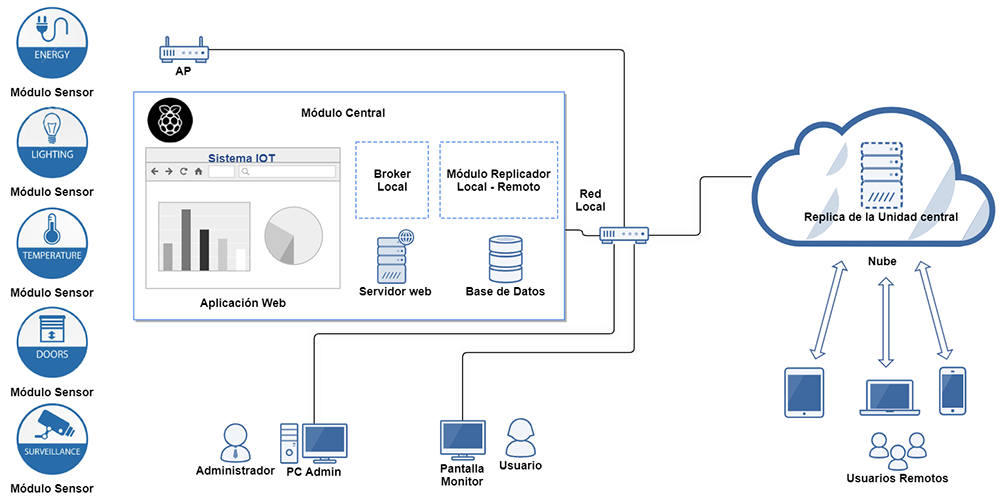
\includegraphics[width=1.07\textwidth]{./Figuras/diagBloques.png}
\caption{Diagrama en bloques del sistema}
\label{fig:diagBloques}
\end{figure}

\vspace{20px}

El sistema IOT a desarrollar contará con componentes esenciales de hardware y software los cuales será necesario desarrollar para poder verificar el funcionamiento del mismo según la idean planteada. 

A continuación se detalla brevemente cada componente que comprende el presente proyecto.

a) MÓDULO PRINCIPAL: Unidad Central Local.
\begin{itemize}
\item Hardware: Raspberry Pi 4.
\item SO: Raspbian.
\item Servidor web: Apache.
\item Base de Datos: MySql
\item Lenguajes Backend: Python, PHP 7.
\item Lenguajes Frontend: HTML5, CSS – Bootstrap 4 y JavaScript.
\item Broker MQTT: Eclipse Mosquitto.
\item Interfaz - Monitor: Pantalla Monitor/Pantalla Touch.
\item Importancia: Este es el módulo principal y el más complejo a desarrollar, es donde se podrá observar un dashboard (resumen) del sistema de control y monitoreo para su acceso en red local. La interfaz gráfica mostrará gráficos estadísticos así como un historial de las lecturas de los sensores y el estado de los mismos.
\end{itemize}

b) MÓDULO REPLICA: Unidad Remota.
\begin{itemize}
\item Servidor web: Apache (Hosting o nube).
\item Base de Datos: MySql.
\item Lenguajes Backend: PHP 7 y JavaScript.
\item Lenguajes FrontEnd: HTML5 y CSS – Bootstrap 4.
\item Importancia: Este es una réplica del módulo principal pero en la nube donde se podrá observar un dashboard del sistema de control y monitoreo pero para el acceso remoto.
\end{itemize}


c) MÓDULO CONSUMO: Para medir Consumo Energético.
\begin{itemize}
\item Hardware Base: NodeMCU esp8266
\item Lenguaje: Arduino.
\item Protocolo Comunicación: MQTT.
\item Sensor: Corriente AC max 100A no invasivo.
\item Medio Transmisión: Wireless.
\item Cantidad: 2
\item Objetos Estudio: Tv y Refrigerador.
\item Importancia: Este módulo permite recoger muestras del valor del consumo diario para poder almacenarlos en la base de datos en el módulo principal, permitiendo estimar costos de consumo mensual; información relevante para el usuario porque permitirá saber el consumo detallado de los dispositivos de estudio.
\end{itemize}

d) MÓDULO TEMPERATURA: Para medir temperatura - Confort.
\begin{itemize}
\item Hardware Base: NodeMCU esp8266
\item Lenguaje: Arduino
\item Protocolo Comunicación: MQTT.
\item Sensor: Temperatura ambiente.
\item Medio Transmisión: Wireless.
\item Cantidad: 2
\item Objetos de Estudio: Sala y una oficina.
\item Importancia: Este módulo permite recoger muestras del valor de la temperatura en determinados ambientes de estudio, dichos valores pueden ser almacenados y usados para estudio de patrones de variación de temperatura por horarios.
\end{itemize}

e) MÓDULO ACTUADOR: Para Control actuador - Confort.
\begin{itemize}
\item Hardware Base: NodeMCU esp8266
\item Lenguaje: Arduino.
\item Protocolo Comunicación: MQTT.
\item Actuador: Relay de un canal.
\item Medio Transmisión: Wireless.
\item Cantidad: 2
\item Objetos de Estudio: Control de Ventiladores (Según datos del Modulo Temperatura).
\item Importancia: Este actuador es un Modulo complementario del "Modulo Temperatura"; permitirá saber el historial de uso y demanda de uso de ventiladores; patrones que pueden ser tema de estudio relacionado al consumo en aplicaciones futuras.
\end{itemize}

f) MÓDULO INTELIGENTE: Para medir y Controlar de forma Inteligente - confort y salud.
\begin{itemize}
\item Hardware Base: Raspberry Pi/Esp32 Cam/Otro.
\item Lenguaje: Arduino y Python.
\item Protocolo Comunicación: MQTT.
\item Actuador: Real-Time Face Recognition.
\item Sensor: Lectura de temperatura corporal.
\item Medio Transmisión: Wireless.
\item Cantidad: 1
\item Objeto de Estudio: Seguimiento de posibles casos de fiebre.
\item Importancia: Este módulo es el segundo módulo complejo a desarrollar por la forma a implementar para la identificación del individuo y la relación de lecturas de temperatura. Con los datos almacenados se puede usar para un estudio de patrones respecto de fechas y estaciones de fiebre. Por el momento se considera en este módulo el tema: "Temperatura corporal", pero para trabajos futuros se puede extender las funcionalidades.
\end{itemize}

\section{Modelo canvas del negocio del proyecto}

El Business Model Canvas, traducido como lienzo de modelo de negocio, es una plantilla de gestión estratégica para el desarrollo de nuevos modelos de negocio y puede resultarles útil para conocer mas a detalle el esquema de negocio. En la Figura \ref{fig:diagCanvas}
es un gráfico visual con elementos que describen la propuesta de negocio del proyecto y los distintos puntos mas importantes respecto a su orientación de mercado.
\vspace{25px}

\begin{figure}[htpb]
\centering 
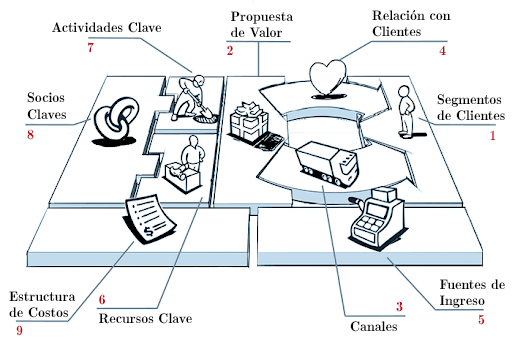
\includegraphics[width=0.75\textwidth]{./Figuras/diagCanvas.png}
\caption{Diagrama del nodelo canvas del negocio}
\label{fig:diagCanvas}
\end{figure}

\begin{enumerate}
\item Segmentos de Cliente:
\begin{itemize}
\item Oficinas, centros educativos, hoteles, centros de salud, edificios de departamentos y centros comerciales.  
\item Familias de clase media y alta.
\end{itemize}
\item Propuesta de valor:
\begin{itemize}
\item Consumo energético detallado por componente eléctrico/electrodoméstico.
\item Control y gestión de confort de distintos ambientes.
\end{itemize}
\item Canales:
   \begin{itemize}
\item Pagina web del producto.
\item Centros comerciales de tecnología.
\item Tiendas de domótica.
\item Empresas que ofrecen soluciones de automatización para hogares, oficinas, etc.
\end{itemize}
\item Relación con Clientes:
\begin{itemize}
\item Centro de información y soporte técnico mediante web.
\item Central telefónica para atender emergencias relacionas al uso del sistema IOT.
\item Una App para dispositivos móviles para solicitar asesoría de uso de los productos o la visita de un técnico. 
\end{itemize}
\item Fuentes de Ingreso:
\begin{itemize}
\item Venta del modulo principal y módulos de sensores básicos.
\item Venta del sistema IOT completo.
\item Venta de módulos se sensado de energía individual con su respectiva App.
\item Pago por consumo de nuestro servicio en la nube.
\end{itemize}
\item Recursos Clave:
\begin{itemize}
\item Diseño pequeño, tecnológico elegante del modulo del sistema principal para usar en casa u otro ambiente.
\item Bajo consumo energético del modulo principal y módulos.
\item Interfaz de usuario amigable y de fácil uso.
\item Sistema seguro y de fácil instalación.
\item Sistema en nube para controlar los brokers remotos de los clientes.
\item Equipo de Investigación y desarrollo.
\item Componentes electrónicos y partes necesarias para la fabricación de módulos.
\end{itemize}
\item Actividades Clave:
\begin{itemize}
\item Estrategias de Marketing.
\item Investigación y Desarrollo.
\item Diseños de presentación de los módulos del sistema.
\item Producción y pruebas de productos.
\item Seguimiento del funcionamiento de los sistemas instalados a clientes.
\item Atención rápida a solicitudes de soporte técnico y asesoría de los productos. 
\end{itemize}
\item Socios Claves:
\begin{itemize}
\item Proveedores de componentes electrónicos y partes necesarias para la fabricación de módulos.
\item Empresas que ofrecen servicios de almacenamiento y gestión de recursos en nube.
\item Tiendas de tecnología y automatización.
\item Centros comerciales de tecnología.
\item Empresas dedicadas a la instalación de soluciones domoticas.
\item Organizadores de eventos y exposiciones de productos tecnológicos.
\end{itemize}
\item Estructura de costos:
\begin{itemize}
\item Costos del equipo de I+D.
\item Costos de fabricación y producción.
\item Costos de almacenamiento y servicios en la nube.
\item Costos por estrategias y ejecución de marketing.
\item Costos por el equipo de atención al cliente.
\item Costos por actividades de desarrollo de negocios (alianzas y convenidos).
\end{itemize}
\end{enumerate}

\section{Identificación y análisis de los interesados}
\label{sec:interesados}

En la siguiente tabla se muestra de  forma resumida los stakeholders del presente proyecto.
\begin{table}[ht]
%\caption{Identificación de los interesados}
%\label{tab:interesados}
\begin{tabularx}{\linewidth}{@{}|l|X|X|l|@{}}
\hline
\rowcolor[HTML]{C0C0C0} 
Rol           & Nombre y Apellido & Organización 	& Puesto 	\\ \hline
Cliente       & \clientename      &\empclientename	&     -   	\\ \hline
Responsable   & \authorname       & FIUBA        	& Alumno 	\\ \hline
Colaboradores &  Docentes y Consultores de hardware y software IOT. &      LSE - FIUBA 	&      Docente 	\\ \hline
Orientador    & \supname	      & \pertesupname 	& Director	Trabajo final \\ \hline
Usuario final & Personas de clase media y alta.\newline    
				Empresas del sector hotelero, salud y cualquier sector comercial. &    -        & Propietario/Jefe \\ \hline


\end{tabularx}
\end{table}

Principales características de cada interesado.

\begin{itemize}
\item Cliente: No existe por el momento un cliente directo dado que es un emprendimiento personal.
\item Responsable: Daniel Iván Cruz Flores, también es el único personal del equipo de desarrollo.
\item Colaboradores: Cada unos de los docentes de la especialización en IOT del LSE - FIUBA.
\item Orientador: \supname, nos va a poder ayudar mucho con la gestión y formulación del proyecto.
\item Usuario Final: Hogares o empresas que desean tener información detalla para gestionar el consumo energético y contar con algunas características de confort.
\end{itemize}

\section{1. Propósito del proyecto}
\label{sec:proposito}

%\begin{consigna}{red}
El proposito de este proyecto es diseñar y desarrollar un sistema informático capaz de controlar y monitorear viviendas u otros ambientes mediante el protocolo MQTT para brindar una gestión inteligente respecto a confort y consumo energético.

%\end{consigna}

\section{2. Alcance del proyecto}
\label{sec:alcance}

Por la cantidad de componentes detallados anteriormente se debe estimar el alcance a considerar para esta primera etapa del proyecto. Se considera un alcance de: 
\begin{itemize}
\item Diseño y desarrollo del Módulo principal.
\item Diseño y desarrollo del Módulo Replica.
\item Diseño y desarrollo del Módulo Consumo.
\item Diseño y desarrollo del Módulo Temperatura.
\item Diseño y desarrollo del Módulo Actuador.
\end{itemize}

El presente proyecto no incluye el desarrollo del ``Módulo Inteligente'' y futuros módulos de interacción por voz Humano - Computador, dichos módulos serán temas de desarrollo en trabajos futuros.

\section{3. Supuestos del proyecto}
\label{sec:supuestos}

\begin{consigna}{red}
``Para el desarrollo del presente proyecto se supone que: ...''
\begin{itemize}
\item Supuesto 1
\item Supuesto 2...
\end{itemize}

%Por ejemplo, se podrían incluir supuestos respecto a disponibilidad de tiempo y recursos humanos y materiales, sobre la factibilidad técnica de distintos aspectos del proyecto, sobre otras cuestiones que sean necesarias para el éxito del proyecto como condiciones macroeconómicas o reglamentarias.

\end{consigna}

\section{4. Requerimientos}
\label{sec:requerimientos}

Los requerimientos se enumeran agrupados por afinidad:

\begin{enumerate}
\item Grupo de requerimientos asociados al "Módulo Principal''.
	\begin{enumerate}
	\item El modulo debe tener instalado un servidor web.
	\item El modulo debe tener instalado un gestor de base de datos MySql.
	\item El modulo debe tener instalado un broker.
	\item El modulo debe tener instalado Pyhton 3.x.
	\item El modulo debe tener un programa ejecutándose en segundo plano para detectar los valores que llegan al broker y enviarlo a la base de datos local.
	\item El modulo debe tener ejecutándose en segundo plano un programa que replicará hacia la nube los datos que reciba el broker local mientras tenga acceso a internet.
	\item El modulo al ser encendido debe iniciar automáticamente el servidor web, el gestor de base de datos, el broker, el programa de captura de datos para el envio a la base de datos y el programa que hace la replica a la nube.
	\item El modulo debe tener una aplicación web para mostrar de forma amigable los datos capturados para permitir la gestión, control y monitoreo del sistema IOT.
	\item La aplicación debe leer los datos que llegan al broker y mostrarlo vía web para comprobar que existe comunicación constante con el resto de módulos del sistema.
	\item La aplicación debe reportar los datos que llegan la base de datos mediante AJAX (Asynchronous JavaScript and XML).
	\item La aplicación debe mostrar información resumida mediante gráficos estadísticos y tablas detalladas de los sensores y módulos del sistema.
	\item La aplicación debe permitir generar reportes detallados en PDF de los datos capturados en la base de datos.
	\item La aplicación debe permitir el acceso de 2 tipos de usuarios: el administrador con permisos totales del sistema y el usuario que solo desea ver información.
	\item La aplicación web deberá seguir funcionando correctamente si existiera algún corte de acceso a internet.
	\item La aplicación debe contar con un protector de pantalla para cuando no se este interactuando (prioridad menor).
	\end{enumerate}
%%%%%%%%%%%%%%%%%%%%%%%%%%%%%%%%%%%%%%%%%%%%%%%%%%%%%%%%%%%%%%%%%%%%%	
\item Grupo de requerimientos asociados al "Módulo Replica''.
	\begin{enumerate}
	\item El modulo debe tener una aplicación web para mostrar de forma amigable los datos replicados del sistema IOT.
	\item La aplicación web estará almacenada en un servicio de servidor web remoto (Hosting).
	\item La aplicación web debe leer todos los datos que llegan al broker remoto de replica.
	\item La aplicación web debe ser estructurada con la característica de adaptabilidad para su acceso desde dispositivos portátiles.
	\item La aplicación deberá mostrar un mensaje de alerta cuando el sistema principal local perdió conexión y no puede enviar los valores en tiempo real.
	\item La aplicación debe permitir el acceso de 2 tipos de usuarios: el administrador con permisos totales del sistema y el usuario que solo desea ver información.
	\end{enumerate}
%%%%%%%%%%%%%%%%%%%%%%%%%%%%%%%%%%%%%%%%%%%%%%%%%%%%%%%%%%%%%%%%%%%%
\item Grupo de requerimientos asociados al "Módulo Consumo''.
	\begin{enumerate}
	\item El modulo debe usar una conexión microUSB para su fuente de alimentación para la placa principal.
	\item El modulo debe leer cada 5 segundos los datos del sensor de corriente.
	\item El modulo debe tener configurado los credenciales necesarios para unirse a la red local mediante Wifi.
	\item El modulo debe enviar sus lecturas obtenidas mediante el protocolo MQTT hacia el broker del Modulo principal central.
	\item El modulo debe estar funcionando 24/7.
	\item El modulo debe tener un case para protección de sus componentes internos y para su mejor presentación (prioridad menor).
	\end{enumerate}	
%%%%%%%%%%%%%%%%%%%%%%%%%%%%%%%%%%%%%%%%%%%%%%%%%%%%%%%%%%%%%%%%%%%%%	
\item Grupo de requerimientos asociados al "Módulo Temperatura''.
	\begin{enumerate}
	\item El modulo debe usar una conexión microUSB para su fuente de alimentación para la placa principal.
	\item El modulo debe leer cada 2 segundos los datos del sensor de temperatura.
	\item El modulo debe tener configurado los credenciales necesarios para unirse a la red local mediante Wifi.
	\item El modulo debe enviar sus lecturas obtenidas mediante el protocolo MQTT hacia el broker del Modulo principal central.
	\item El modulo debe estar funcionando 24/7.
	\item El modulo debe tener un case para protección de sus componentes internos y para su mejor presentación(prioridad menor)
	\end{enumerate}	
%%%%%%%%%%%%%%%%%%%%%%%%%%%%%%%%%%%%%%%%%%%%%%%%%%%%%%%%%%%%%%%%%%%%%
\item Grupo de requerimientos asociados al "Módulo Actuador''.
	\begin{enumerate}
	\item El modulo debe usar una conexión microUSB para su fuente de alimentación para la placa principal.
		\item El modulo debe recibir datos mediante el protocolo MQTT desde el broker del Modulo principal central.
	\item El modulo debe leer cada 1 segundos los datos que se le envían desde el modulo principal.
	\item El modulo debe tener configurado los credenciales necesarios para unirse a la red local mediante Wifi.
	\item El modulo debe estar funcionando 24/7.
	\item El modulo deberá estar conectado a un ventilador y actuara mediante un rele para su encendido o apagado del mismo.
	\item El modulo debe tener un case para protección de sus componentes internos y para su mejor presentación(prioridad menor)
	\end{enumerate}

\item Grupo de requerimientos asociados a la ''Red Local''.
	\begin{enumerate}
	\item La red local debe estar configurado con direcciones Ip estáticas.
	\item La red local debe estar configurado con un Access Point para garantizar la fácil conexión entre módulos del sistema IOT así como extender el rango de la señal wifi.
	\item El Access Point de la red debe estar configurado en un canal de comunicación que no tenga solapamiento de canales wifi.
	\item La conexión a la red del pc del usuario administrador y de la pantalla monitor debe estar conectado vía cable Ethernet(prioridad menor).
	\end{enumerate}

\end{enumerate}

\section{Historias de usuarios (\textit{Product backlog})}
\label{sec:backlog}

\begin{consigna}{red}
Descripción: En esta sección se deben incluir las historias de usuarios y su ponderación (\textit{history points}). Recordar que las historias de usuarios son descripciones cortas y simples de una característica contada desde la perspectiva de la persona que desea la nueva capacidad, generalmente un usuario o cliente del sistema. La ponderación es un número entero que representa el tamaño de la historia comparada con otras historias de similar tipo.
\end{consigna}

\section{5. Entregables principales del proyecto}
\label{sec:entregables}
Para la verificación del funcionamiento del sistema IOT a implementar se considera los siguientes recursos entregables:
\begin{itemize}
\item Manual de uso.
\item Diagrama esquemático.
\item Diagrama de los componentes que forman el sistema.
\item Vídeo demostrativo de las pruebas de funcionamiento.
\item Informe final.

\end{itemize}

\section{6. Desglose del trabajo en tareas}
\label{sec:wbs}
Las tareas se muestras agrupados para una mejor comprensión:
%%%%%%%%%%%%%%%%%%%%%%%%%%%%%%%%%%%%%%%%%%%%%%%%%%%%%%%%%%%%%%%%%%%%%%%%%%
\begin{enumerate}
\item Búsqueda de material bibliográfico. (58 hs)
	\begin{enumerate}
	\item Búsqueda de soluciones similares en el mercado. (5 hs)
	\item Búsqueda de códigos fuente similares a los que se usará. (10 hs)
	\item Búsqueda de todos los componentes electrónicos a usar. (10 hs)
	\item Estudiar la forma de integración de componentes a la red. (10 hs)
	\item Estudiar cómo funciona cada uno de los componentes. (15 hs)
	\item Realizar un informe resumen con la lista de componentes, aspectos de red y configuraciones básicas a usar. (8 hs)
	\end{enumerate}
\item Adquisición de componentes. (20 hs)
	\begin{enumerate}
	\item Cotizar los costos de cada componente electrónico con los proveedores. (8 hs)
	\item Realizar los pedidos a proveedores. (4 hs)
	\item Realizar un informe de costos de los componentes adquiridos (8 hs)
	\end{enumerate}
%%%%%%%%%%%%%%%%%%%%%%%%%%%%%%%%%%%%%%%%%%%%%%%%%%%%%%%%%%%%%%%%%%%%%%%%%%%%%
\item Diseño y configuración de Red Local. (24 hs)
	\begin{enumerate}
	\item Instalación del Modem/router en el lugar mas adecuado. (3 hs)
	\item Instalación del Access Point en el lugar mas adecuado. (4 hs)
	\item Configuración interna del Modem/Router y el Access Point. (4 hs)
	\item Verificación e instalación de los puntos de donde se conectaran los módulos sensores de muestreo. (5 hs)
	\item Realizar un informe de la configuración de red local instalada. (8 hs)
	\end{enumerate}
%%%%%%%%%%%%%%%%%%%%%%%%%%%%%%%%%%%%%%%%%%%%%%%%%%%%%%%%%%%%%%%%%%%%%%%%%%%%%
\item Desarrollo del Modulo Principal. (252 hs)
	\begin{enumerate}
	\item Instalación del sistema operativo en la Raspberry Pi (2 hs)
	\item Instalación y configuración del servidor web (5 hs)
	\item Instalación y configuración de Python 3 (2 hs)
	\item Instalación y configuración del Broker Local (5 hs)
	\item Creación del programa para leer datos que llegan al broker y enviarlo a la base de datos. (5 hs)
	\item Creación del programa para verificar constantemente el acceso a internet (5 hs)
	\item Creación del programa para leer datos que llegan al broker y replicarlos a la nube. (15 hs)
	\item Creación y configuración del script lanzador que iniciará automáticamente los programas al encender el modulo. (10 hs)
	\item Testeo del funcionamiento y conexión a la red inicial del modulo. (10 hs)
	\item Diseño y creación de la base de datos. (10 hs)
	\item Diseño y maquetación de la aplicación web principal. (35 hs)
	\item Desarrollo de todas las funcionalidades backend de la aplicación. (40 hs)
	\item Integración de todas las funcionalidades backend con el fronted de la aplicación web (30 hs)
	\item Creación de los tipos de reportes que ofrecerá la aplicación. (20 hs)
	\item Testeo y depuración del funcionamiento de los roles de acceso al sistema. (10 hs)
	\item Testeo y depuración del funcionamiento de la aplicación web en el pc del administrador. (5 hs)
	\item Testeo y depuración del funcionamiento de la aplicación web en el monitor informativo. (5 hs)
	\item Testeo y depuración del funcionamiento del sistema del modulo principal en situaciones de corte de internet. (30 hs) 
	\item Realizar un informe resumen de las características del modulo, aspectos de red, configuraciones a usar, credenciales de acceso del usuario root, versiones del software, credenciales de acceso a la administración a la base de datos y a la aplicación web. (8 hs)
	\end{enumerate}
%%%%%%%%%%%%%%%%%%%%%%%%%%%%%%%%%%%%%%%%%%%%%%%%%%%%%%%%%%%%%%%%%%%%%%%%%%%%%%%%
\item Desarrollo del Modulo Replica. (143 hs)
	\begin{enumerate}
	\item Creación y configuración del Broker remoto (5 hs)
	\item Integración del Broker remoto con el modulo principal local para las replicas(10 hs)
	\item verificación y testeo de enlace del broker local con el broker remoto. (10 hs)
	\item Creación de la base de datos replica en la nube. (5 hs) 
	\item Adaptación de la aplicación web local para su funcionamiento en remoto  (40 hs)
	\item Configuración de recepción de datos del broker remoto hacia la aplicación en nube.  (20 hs)
	\item Testeo y depuración del funcionamiento de los roles de acceso al sistema. (10 hs) 
	\item Testeo y depuración del funcionamiento de la aplicación web desde el pc del administrador. (5 hs) 
	\item Testeo y depuración del funcionamiento de la aplicación en diferentes dispositivos portátiles. (30 hs)
	\item Realizar un informe resumen de las configuraciones a usar y credenciales de acceso a la cuenta de administración. (8 hs)
	\end{enumerate}
%%%%%%%%%%%%%%%%%%%%%%%%%%%%%%%%%%%%%%%%%%%%%%%%%%%%%%%%%%%%%%%%%%%%%%%%%%%%%%%%%
\item Desarrollo del Modulo de Consumo. (73 hs)
	\begin{enumerate}
	\item Construcción del modulo e integración de componentes, sensor de corriente con placa Esp8266. (15 hs)
	\item Creación del programa de lectura para el microcontrolador. (15 hs)
	\item Testeo de conexión del modulo a la red y al modulo principal central. (10 hs)
	\item Testeo y depuración del envió de datos al modulo principal de la red local. (10 hs)
	\item Verificación y formateo de datos capturados por el sensor para su envió al modulo central. (10 hs)
	\item Instalación del modulo en un ambiente determinado para su funcionamiento. (5 hs)
	\item Realizar un informe resumen de las configuraciones a usar, código fuente e información respecto al formato de envió de datos. (8 hs)
	\end{enumerate}
%%%%%%%%%%%%%%%%%%%%%%%%%%%%%%%%%%%%%%%%%%%%%%%%%%%%%%%%%%%%%%%%%%%%%%%%%%%%%%%%%%%
\item Desarrollo del Modulo Temperatura. (68 hs)
	\begin{enumerate}
	\item Construcción del modulo e integración de componentes, sensor de temperatura con placa Esp8266. (15 hs)
	\item Creación del programa de lectura para el microcontrolador. (15 hs)
	\item Testeo de conexión del modulo a la red y al modulo principal central. (10 hs)
	\item Testeo y depuración del envió de datos al modulo principal de la red local. (10 hs)
	\item Verificación y formateo de datos capturados por el sensor para su envió al modulo central. (5 hs)
	\item Instalación del modulo en un ambiente determinado para su funcionamiento. (5 hs)
	\item Realizar un informe resumen de las configuraciones a usar, código fuente e información respecto al formato de envió de datos. (8 hs)
	\end{enumerate}
%%%%%%%%%%%%%%%%%%%%%%%%%%%%%%%%%%%%%%%%%%%%%%%%%%%%%%%%%%%%%%%%%%%%%%%%%%%%%%%%%%%%
\item Desarrollo del Modulo Actuador. (88 hs)
	\begin{enumerate}
	\item Construcción del modulo e integración de componentes, actuador con placa Esp8266. (15 hs)
	\item Creación del programa de lectura para el microcontrolador. (15 hs)
	\item Testeo de conexión del modulo a la red y al modulo principal central. (10 hs)
	\item Testeo y depuración de la recepción y envió de datos al modulo principal de la red local. (20 hs)
	\item Verificación y formateo de datos capturados de la red para su manipulación y transformación en ordenes de la placa hacia el Rele.(15 hs)
	\item Instalación del modulo en un ambiente determinado para su funcionamiento. (5 hs)
	\item Realizar un informe resumen de las configuraciones a usar, código fuente e información respecto al formato de recepción de datos. (8 hs)
	\end{enumerate}
%%%%%%%%%%%%%%%%%%%%%%%%%%%%%%%%%%%%%%%%%%%%%%%%%%%%%%%%%%%%%%%%%%%%%%%%%%%%%%%%%%%%%
\item Verificación y testeo del sistema IOT. (68 hs)
	\begin{enumerate}
	\item Verificación y depuración del funcionamiento completo del sistema IOT en un ambiente de red local controlado (laboratorio) con acceso a internet (10 hs)
	\item Verificación y depuración del funcionamiento de los roles de acceso del sistema IOT en un ambiente de red local controlado (laboratorio) con acceso a internet (10 hs) 
	\item Verificación y depuración del funcionamiento completo del sistema IOT en un ambiente real con acceso a internet vía red local(10 hs) 
	\item Verificación y depuración del funcionamiento completo del sistema IOT en un ambiente real sin acceso a internet vía red local (10 hs) 
	\item Verificación y depuración del funcionamiento completo del sistema replica IOT remoto desde un dispositivo portátil (10 hs)
	\item Verificación y depuración del funcionamiento completo del sistema replica IOT remoto desde un dispositivo portátil cuando el modulo principal local se desconecta de internet (10 hs)
	\item Realizar un informe resumen con las correcciones de las nuevas configuraciones a usar y todas las nuevas consideraciones de funcionamiento. (8 hs)
	\end{enumerate}
%%%%%%%%%%%%%%%%%%%%%%%%%%%%%%%%%%%%%%%%%%%%%%%%%%%%%%%%%%%%%%%%%%%%%%%%%%%%%%%%%%%%%	
\item Propuestas y recomendaciones de mejora para la presentación del sistema IOT. (35 hs)
	\begin{enumerate}
	\item Creación de propuestas de mejora en el aspecto de presentación física para el modulo principal (5 hs)
	\item Creación de propuestas de mejora en el aspecto de presentación física para cada uno de los módulos (5 hs)
	\item Creación de propuestas de mejora para nuevas funcionalidades a considerar para su integración en trabajos futuros(5 hs)
	\item Creación del manual de usuario del sistema IOT. (10 hs)
	\item Creación de un vídeo resumen explicativo comercial del funcionamiento del sistema (10 hs)
	\end{enumerate}	
		
\end{enumerate}

Cantidad total de horas: (794 hs)

\section{7. Diagrama de Activity On Node}
\label{sec:AoN}

\begin{consigna}{red}
Armar el AoN a partir del WBS definido en la etapa anterior. 

%La figura \ref{fig:AoN} fue elaborada con el paquete latex tikz y pueden consultar la siguiente referencia \textit{online}:

%\url{https://www.overleaf.com/learn/latex/LaTeX_Graphics_using_TikZ:_A_Tutorial_for_Beginners_(Part_3)\%E2\%80\%94Creating_Flowcharts}

\end{consigna}

\begin{figure}[htpb]
\centering 
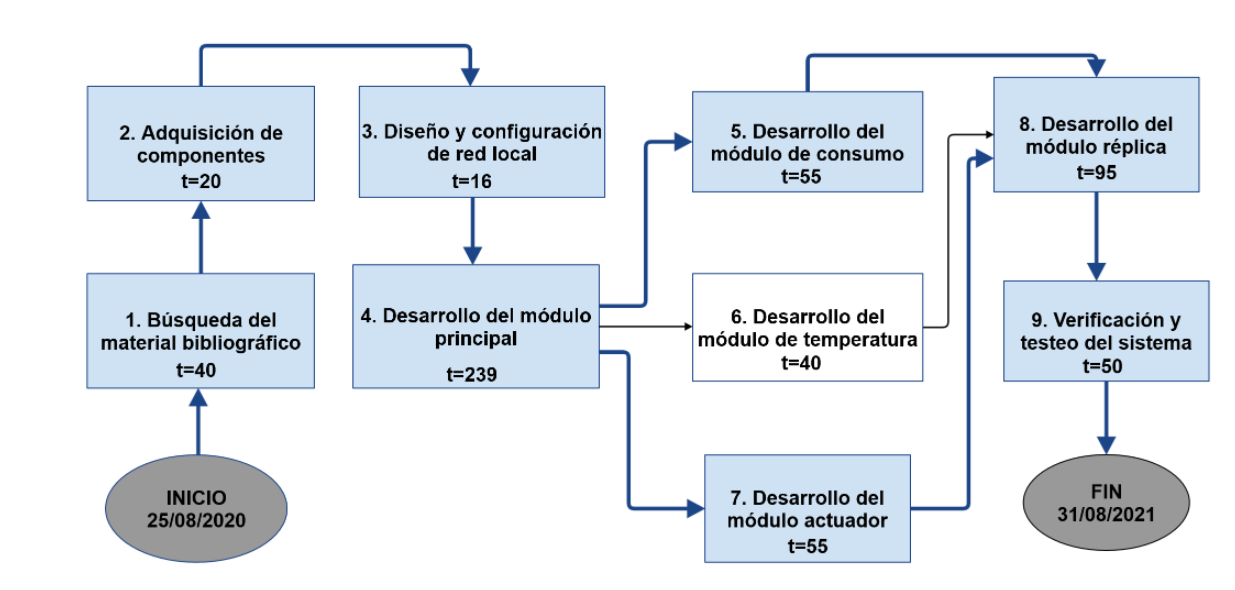
\includegraphics[width=.8\textwidth]{./Figuras/AoN.png}
\caption{Diagrama en \textit{Activity on Node}}
\label{fig:AoN}
\end{figure}

Indicar claramente en qué unidades están expresados los tiempos.
De ser necesario indicar los caminos semicríticos y analizar sus tiempos mediante un cuadro.
Es recomendable usar colores y un cuadro indicativo describiendo qué representa cada color, como se muestra en el siguiente ejemplo:



\section{8. Diagrama de Gantt}
\label{sec:gantt}

\begin{consigna}{red}
Utilizar el software Gantter for Google Drive o alguno similar para dibujar el diagrama de Gantt.

Existen muchos programas y recursos \textit{online} para hacer diagramas de gantt, entre las cuales destacamos:

\begin{itemize}
\item Planner
\item GanttProject
\item Trello + \textit{plugins}. En el siguiente link hay un tutorial oficial: \\ \url{https://blog.trello.com/es/diagrama-de-gantt-de-un-proyecto}
\item Creately, herramienta online colaborativa. \\\url{https://creately.com/diagram/example/ieb3p3ml/LaTeX}
\item Se puede hacer en latex con el paquete \textit{pgfgantt}\\ \url{http://ctan.dcc.uchile.cl/graphics/pgf/contrib/pgfgantt/pgfgantt.pdf}
\end{itemize}

Pegar acá una captura de pantalla del diagrama de Gantt, cuidando que la letra sea suficientemente grande como para ser legible. 
Si el diagrama queda demasiado ancho, se puede pegar primero la ``tabla'' del Gantt y luego pegar la parte del diagrama de barras del diagrama de Gantt.

Configurar el software para que en la parte de la tabla muestre los códigos del EDT (WBS).\\
Configurar el software para que al lado de cada barra muestre el nombre de cada tarea.\\
Revisar que la fecha de finalización coincida con lo indicado en el Acta Constitutiva.

En la figura \ref{fig:gantt}, se muestra un ejemplo de diagrama de gantt realizado con el paquete de \textit{pgfgantt}. En la plantilla pueden ver el código que lo genera y usarlo de base para construir el propio.

\begin{figure}[htbp]
\begin{center}
\begin{ganttchart}{1}{12}
  \gantttitle{2020}{12} \\
  \gantttitlelist{1,...,12}{1} \\
  \ganttgroup{Group 1}{1}{7} \\
  \ganttbar{Task 1}{1}{2} \\
  \ganttlinkedbar{Task 2}{3}{7} \ganttnewline
  \ganttmilestone{Milestone o hito}{7} \ganttnewline
  \ganttbar{Final Task}{8}{12}
  \ganttlink{elem2}{elem3}
  \ganttlink{elem3}{elem4}
\end{ganttchart}
\end{center}
\caption{Diagrama de gantt de ejemplo}
\label{fig:gantt}
\end{figure}

\end{consigna}

\section{9. Matriz de uso de recursos de materiales}
\label{sec:recursos}


\begin{table}
\label{tab:recursos}
\centering
\begin{tabularx}{\linewidth}{@{}|c|X|X|X|X|c|@{}}
\hline
\cellcolor[HTML]{C0C0C0} & \cellcolor[HTML]{C0C0C0} & \multicolumn{4}{c|}{\cellcolor[HTML]{C0C0C0}Recursos requeridos (horas)} \\ \cline{3-6} 
\multirow{-2}{*}{\cellcolor[HTML]{C0C0C0}\begin{tabular}[c]{@{}c@{}}Código\\ WBS\end{tabular}} & \multirow{-2}{*}{\cellcolor[HTML]{C0C0C0}\begin{tabular}[c]{@{}c@{}}Nombre \\ tarea\end{tabular}} & Material 1 & Material 2 & Material 3 & Material 4 \\ \hline
 &  &  &  &  &  \\ \hline
 &  &  &  &  &  \\ \hline
 &  &  &  &  &  \\ \hline
 &  &  &  &  &  \\ \hline
 &  &  &  &  &  \\ \hline
 &  &  &  &  &  \\ \hline
 &  &  &  &  &  \\ \hline
 &  &  &  &  &  \\ \hline 
 &  &  &  &  &  \\ \hline
 &  &  &  &  &  \\ \hline
 &  &  &  &  &  \\ \hline
 &  &  &  &  &  \\ \hline
 &  &  &  &  &  \\ \hline
 &  &  &  &  &  \\ \hline
 &  &  &  &  &  \\ \hline
 &  &  &  &  &  \\ \hline
 &  &  &  &  &  \\ \hline
 &  &  &  &  &  \\ \hline
 &  &  &  &  &  \\ \hline
 &  &  &  &  &  \\ \hline
 &  &  &  &  &  \\ \hline
 &  &  &  &  &  \\ \hline
 &  &  &  &  &  \\ \hline
 &  &  &  &  &  \\ \hline 
 &  &  &  &  &  \\ \hline
 &  &  &  &  &  \\ \hline
 &  &  &  &  &  \\ \hline
 &  &  &  &  &  \\ \hline

\end{tabularx}%
\end{table}


\section{10. Presupuesto detallado del proyecto}
\label{sec:presupuesto}

\begin{consigna}{red}
Si el proyecto es complejo entonces separarlo en partes:
\begin{itemize}
\item Un total global, indicando el subtotal acumulado por cada una de las áreas.
\item El desglose detallado del subtotal de cada una de las áreas.
\end{itemize}

IMPORTANTE: No olvidarse de considerar los COSTOS INDIRECTOS.

\end{consigna}

\begin{table}[htpb]
\centering
\begin{tabularx}{\linewidth}{@{}|X|c|r|r|@{}}
\hline
\rowcolor[HTML]{C0C0C0} 
\multicolumn{4}{|c|}{\cellcolor[HTML]{C0C0C0}COSTOS DIRECTOS} \\ \hline
\rowcolor[HTML]{C0C0C0} 
Descripción &
  \multicolumn{1}{c|}{\cellcolor[HTML]{C0C0C0}Cantidad} &
  \multicolumn{1}{c|}{\cellcolor[HTML]{C0C0C0}Valor unitario} &
  \multicolumn{1}{c|}{\cellcolor[HTML]{C0C0C0}Valor total} \\ \hline
 &
  \multicolumn{1}{c|}{} &
  \multicolumn{1}{c|}{} &
  \multicolumn{1}{c|}{} \\ \hline
 &
  \multicolumn{1}{c|}{} &
  \multicolumn{1}{c|}{} &
  \multicolumn{1}{c|}{} \\ \hline
\multicolumn{1}{|l|}{} &
   &
   &
   \\ \hline
\multicolumn{1}{|l|}{} &
   &
   &
   \\ \hline
\multicolumn{3}{|c|}{SUBTOTAL} &
  \multicolumn{1}{c|}{} \\ \hline
\rowcolor[HTML]{C0C0C0} 
\multicolumn{4}{|c|}{\cellcolor[HTML]{C0C0C0}COSTOS INDIRECTOS} \\ \hline
\rowcolor[HTML]{C0C0C0} 
Descripción &
  \multicolumn{1}{c|}{\cellcolor[HTML]{C0C0C0}Cantidad} &
  \multicolumn{1}{c|}{\cellcolor[HTML]{C0C0C0}Valor unitario} &
  \multicolumn{1}{c|}{\cellcolor[HTML]{C0C0C0}Valor total} \\ \hline
\multicolumn{1}{|l|}{} &
   &
   &
   \\ \hline
\multicolumn{1}{|l|}{} &
   &
   &
   \\ \hline
\multicolumn{1}{|l|}{} &
   &
   &
   \\ \hline
\multicolumn{3}{|c|}{SUBTOTAL} &
  \multicolumn{1}{c|}{} \\ \hline
\rowcolor[HTML]{C0C0C0}
\multicolumn{3}{|c|}{TOTAL} &
   \\ \hline
\end{tabularx}%
\end{table}


\section{11. Matriz de asignación de responsabilidades}
\label{sec:responsabilidades}
\begin{consigna}{red}
Establecer la matriz de asignación de responsabilidades y el manejo de la autoridad completando la siguiente tabla:

\begin{table}[htpb]
\centering
\resizebox{\textwidth}{!}{%
\begin{tabular}{|c|c|c|c|c|c|}
\hline
\rowcolor[HTML]{C0C0C0} 
\cellcolor[HTML]{C0C0C0} &
  \cellcolor[HTML]{C0C0C0} &
  \multicolumn{4}{c|}{\cellcolor[HTML]{C0C0C0}Listar todos los nombres y roles del proyecto} \\ \cline{3-6} 
\rowcolor[HTML]{C0C0C0} 
\cellcolor[HTML]{C0C0C0} &
  \cellcolor[HTML]{C0C0C0} &
  Responsable &
  Orientador &
  Equipo &
  Cliente \\ \cline{3-6} 
\rowcolor[HTML]{C0C0C0} 
\multirow{-3}{*}{\cellcolor[HTML]{C0C0C0}\begin{tabular}[c]{@{}c@{}}Código\\ WBS\end{tabular}} &
  \multirow{-3}{*}{\cellcolor[HTML]{C0C0C0}Nombre de la tarea} &
  \authorname &
  \supname &
  Nombre de alguien &
  \clientename \\ \hline
 &  &  &  &  &  \\ \hline
 &  &  &  &  &  \\ \hline
 &  &  &  &  &  \\ \hline
\end{tabular}%
}
\end{table}

{\footnotesize
Referencias:
\begin{itemize}
	\item P = Responsabilidad Primaria
	\item S = Responsabilidad Secundaria
	\item A = Aprobación
	\item I = Informado
	\item C = Consultado
\end{itemize}
} %footnotesize

Una de las columnas debe ser para el Director, ya que se supone que participará en el proyecto.
A su vez se debe cuidar que no queden muchas tareas seguidas sin ``A'' o ``I''.

Importante: es redundante poner ``I/A'' o ``I/C'', porque para aprobarlo o responder consultas primero la persona debe ser informada.

\end{consigna}

\section{12. Gestión de riesgos}
\label{sec:riesgos}

\begin{consigna}{red}
a) Identificación de los riesgos (al menos cinco) y estimación de sus consecuencias:
 
Riesgo 1: detallar el riesgo (riesgo es algo que si ocurre altera los planes previstos)
\begin{itemize}
\item Severidad (S): mientras más severo, más alto es el número (usar números del 1 al 10).\\
Justificar el motivo por el cual se asigna determinado número de severidad (S).
\item Probabilidad de ocurrencia (O): mientras más probable, más alto es el número (usar del 1 al 10).\\
Justificar el motivo por el cual se asigna determinado número de (O). 
\end{itemize}   

Riesgo 2:
\begin{itemize}
\item Severidad (S): 
\item Ocurrencia (O):
\end{itemize}

Riesgo 3:
\begin{itemize}
\item Severidad (S): 
\item Ocurrencia (O):
\end{itemize}


b) Tabla de gestión de riesgos:      (El RPN se calcula como RPN=SxO)

\begin{table}[htpb]
\centering
\begin{tabularx}{\linewidth}{@{}|X|c|c|c|c|c|c|@{}}
\hline
\rowcolor[HTML]{C0C0C0} 
Riesgo & S & O & RPN & S* & O* & RPN* \\ \hline
       &   &   &     &    &    &      \\ \hline
       &   &   &     &    &    &      \\ \hline
       &   &   &     &    &    &      \\ \hline
       &   &   &     &    &    &      \\ \hline
       &   &   &     &    &    &      \\ \hline
\end{tabularx}%
\end{table}

Criterio adoptado: 
Se tomarán medidas de mitigación en los riesgos cuyos números de RPN sean mayores a...

Nota: los valores marcados con (*) en la tabla corresponden luego de haber aplicado la mitigación.

c) Plan de mitigación de los riesgos que originalmente excedían el RPN máximo establecido:
 
Riesgo 1: plan de mitigación (si por el RPN fuera necesario elaborar un plan de mitigación).
  Nueva asignación de S y O, con su respectiva justificación:
  - Severidad (S): mientras más severo, más alto es el número (usar números del 1 al 10).
          Justificar el motivo por el cual se asigna determinado número de severidad (S).
  - Probabilidad de ocurrencia (O): mientras más probable, más alto es el número (usar del 1 al 10).
          Justificar el motivo por el cual se asigna determinado número de (O).

Riesgo 2: plan de mitigación (si por el RPN fuera necesario elaborar un plan de mitigación).
 
Riesgo 3: plan de mitigación (si por el RPN fuera necesario elaborar un plan de mitigación).

\end{consigna}


\section{13. Gestión de la calidad}
\label{sec:calidad}

\begin{consigna}{red}
Para cada uno de los requerimientos del proyecto indique:
\begin{itemize} 
\item Req \#1: copiar acá el requerimiento.

Verificación y validación:

\begin{itemize}
\item Verificación para confirmar si se cumplió con lo requerido antes de mostrar el sistema al cliente. Detallar 
\item Validación con el cliente para confirmar que está de acuerdo en que se cumplió con lo requerido. Detallar  
\end{itemize}

\end{itemize}

Tener en cuenta que en este contexto se pueden mencionar simulaciones, cálculos, revisión de hojas de datos, consulta con expertos, mediciones, etc.

\end{consigna}

\section{14. Comunicación del proyecto}
\label{sec:comunicaciones}

El plan de comunicación del proyecto es el siguiente:

\begin{table}[htpb]
\centering
\begin{tabularx}{\linewidth}{@{}|X|C{2.4cm}|C{3cm}|C{1.8cm}|C{2cm}|C{2.1cm}|@{}}
\hline
\rowcolor[HTML]{C0C0C0} 
\multicolumn{6}{|c|}{\cellcolor[HTML]{C0C0C0}PLAN DE COMUNICACIÓN DEL PROYECTO}           \\ \hline
\rowcolor[HTML]{C0C0C0} 
¿Qué comunicar? & Audiencia & Propósito & Frecuencia & Método de comunicac. & Responsable \\ \hline
                &           &           &            &                      &             \\ \hline
                &           &           &            &                      &             \\ \hline
                &           &           &            &                      &             \\ \hline
                &           &           &            &                      &             \\ \hline
                &           &           &            &                      &             \\ \hline
\end{tabularx}
\end{table}

\section{15. Gestión de compras}
\label{sec:compras}

\begin{consigna}{red}
En caso de tener que comprar elementos o contratar servicios:
a) Explique con qué criterios elegiría a un proveedor.
b) Redacte el Statement of Work correspondiente.
\end{consigna}

\section{16. Seguimiento y control}
\label{sec:seguimiento}

\begin{consigna}{red}
Para cada tarea del proyecto establecer la frecuencia y los indicadores con los se seguirá su avance y quién será el responsable de hacer dicho seguimiento y a quién debe comunicarse la situación (en concordancia con el Plan de Comunicación del proyecto).

El indicador de avance tiene que ser algo medible, mejor incluso si se puede medir en \% de avance. Por ejemplo,se pueden indicar en esta columna cosas como ``cantidad de conexiones ruteadeas'' o ``cantidad de funciones implementadas'', pero no algo genérico y ambiguo como ``\%'', porque el lector no sabe porcentaje de qué cosa.

\end{consigna}

\begin{longtable}{|m{1cm}|m{3.5cm}|m{2.2cm}|m{2cm}|m{3cm}|m{1.5cm}|}
\hline
\rowcolor[HTML]{C0C0C0} 
\multicolumn{6}{|c|}{\cellcolor[HTML]{C0C0C0}SEGUIMIENTO DE AVANCE}                                                                       \\ \hline
\rowcolor[HTML]{C0C0C0} 
Tarea del WBS 			& Indicador de avance & Frecuencia de reporte & Resp. de seguimiento & Persona a ser informada & Método de comunic. \\ \hline
\endfirsthead

\hline
\rowcolor[HTML]{C0C0C0} 
\multicolumn{6}{c}{\cellcolor[HTML]{C0C0C0}SEGUIMIENTO DE AVANCE}                                                                       \\ \hline
\rowcolor[HTML]{C0C0C0} 
Tarea del WBS 			& Indicador de avance & Frecuencia de reporte & Resp. de seguimiento & Persona a ser informada & Método de comunic. \\ \hline
\endhead

\multicolumn{6}{c}{Continúa}
\endfoot

\endlastfoot

1.1	& Fecha de inicio  & Única vez al comienzo & \authorname & \clientename, \supname & email \\ \hline
2.1	& Avance de las subtareas  & Mensual mientras dure la tarea & \authorname & \clientename, \supname & email \\ \hline

\end{longtable}

\begin{table}[!htpb]
\centering
%\begin{tabularx}{\linewidth}{@{}|X|X|X|X|X|X|@{}}
\begin{tabularx}{\linewidth}{@{}|X|C{2.5cm}|C{3cm}|C{2cm}|C{2cm}|C{2.5cm}|@{}}
\hline
\rowcolor[HTML]{C0C0C0} 
\multicolumn{6}{|c|}{\cellcolor[HTML]{C0C0C0}SEGUIMIENTO DE AVANCE}                                                                       \\ \hline
\rowcolor[HTML]{C0C0C0} 
Tarea del WBS & Indicador de avance & Frecuencia de reporte & Resp. de seguimiento & Persona a ser informada & Método de comunic. \\ \hline
 &  &  &  &  &  \\ \hline
 &  &  &  &  &  \\ \hline
 &  &  &  &  &  \\ \hline
 &  &  &  &  &  \\ \hline
 &  &  &  &  &  \\ \hline
\end{tabularx}%
%}
\end{table}

\section{17. Procesos de cierre}    
\label{sec:cierre}

\begin{consigna}{red}
Establecer las pautas de trabajo para realizar una reunión final de evaluación del proyecto, tal que contemple las siguientes actividades:

\begin{itemize}
\item Pautas de trabajo que se seguirán para analizar si se respetó el Plan de Proyecto original:
 - Indicar quién se ocupará de hacer esto y cuál será el procedimiento a aplicar. 
\item Identificación de las técnicas y procedimientos útiles e inútiles que se utilizaron, y los problemas que surgieron y cómo se solucionaron:
 - Indicar quién se ocupará de hacer esto y cuál será el procedimiento para dejar registro.
\item Indicar quién organizará el acto de agradecimiento a todos los interesados, y en especial al equipo de trabajo y colaboradores:
  - Indicar esto y quién financiará los gastos correspondientes.
\end{itemize}

\end{consigna}


\end{document}
